\documentclass[11pt, oneside]{article}   	% use "amsart" instead of "article" for AMSLaTeX format
\usepackage{geometry}                		% See geometry.pdf to learn the layout options. There are lots.
\geometry{letterpaper}                   		% ... or a4paper or a5paper or ... 

\usepackage[english]{babel}
\usepackage{url, verse}
\usepackage{pstricks, tikz}
\usepackage[T1]{fontenc}
\usepackage{setspace}
\usepackage{graphicx, wrapfig, capt-of}
\usepackage[normalem]{ulem} %for \sout
\usepackage{amssymb}
\usepackage{color}
\usepackage{tipa}
\usepackage{multicol}

\usepackage{stackengine}
\usepackage{array}
\newcolumntype{P}[1]{>{\centering\arraybackslash}p{#1}}
\newcolumntype{M}[1]{>{\centering\arraybackslash}m{#1}}
\usepackage{hhline,multirow}
\newcommand*\rot{\rotatebox{90}}

\usepackage{linguex} %declare this package after tipa and graphicx
\renewcommand{\firstrefdash}{}
\usepackage{qtree}
\usepackage{tree-dvips} %copy tree-dvips folder to make this work
\qtreecenterfalse

\usepackage{float}
\usepackage{tcolorbox, enumitem}
\usepackage{phonrule}

\usepackage{fancyhdr}
\pagestyle{fancy}{
\fancyhead[L]{Roberto Petrosino}
\fancyhead[C]{LING2010Q}
\fancyhead[R]{3: Phonology}
\renewcommand{\footrulewidth}{0pt}
\renewcommand{\headrulewidth}{0pt}}

\newenvironment{packed_enum}{
\begin{enumerate}
  \setlength{\itemsep}{1pt}
  \setlength{\parskip}{0pt}
  \setlength{\parsep}{0pt}
}{\end{enumerate}}

\newenvironment{packed_item}{
\begin{itemize}
  \setlength{\itemsep}{1pt}
  \setlength{\parskip}{0pt}
  \setlength{\parsep}{0pt}
}{\end{itemize}}

\renewcommand{\labelitemiii}{$\diamond$}


\title{{\normalsize LING 2010Q -- {\scshape Spring 2017}} \\ {\bfseries 3 - Phonology}, or: \\ {\itshape the science of sounds -- level of abstractness: 1 -- $\infty$}}
\author{Roberto Petrosino \hspace{0.2cm} \url{roberto.petrosino@uconn.edu}}
\date{September 19-28, 2017}

\begin{document}

\maketitle
\tableofcontents

\newpage

\section{Some basic definitions - recap}

\ex. {\bfseries Phonetics} studies every linguistic sound that humans can possibly produce with the vocal tract, from a purely articulatory point of view. This is superset A. 
\a. {\bfseries Articulatory phonetics} studies the physiology of how speech sounds/signs are produced. 
\b. {\bfseries Acoustic phonetics} studies the physical properties of speech sounds. 
\c. {\bfseries Auditory phonetics} deals with how speech sounds are perceived.

\ex. In the set B of {\itshape all possible linguistic sounds}, a subset of A, {\bfseries phonology} studies the subset of linguistic sounds $\beta$ chosen by a specific language to form words; languages may or may not share some sounds. Phonology also concerns with how sounds are put together to form syllables and words. We will deal with phonology in the next module. 

\begin{figure}[H]
\centering
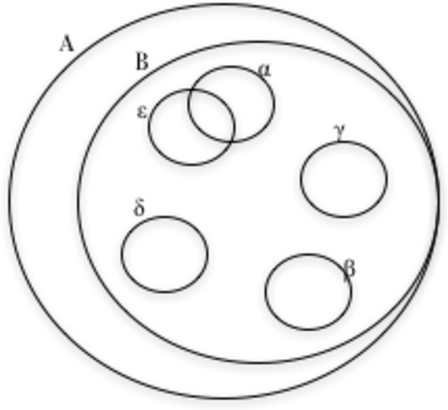
\includegraphics[scale=0.9]{sounds_sets}
\end{figure}%

\newpage

\section{Abstractness level 1 -- {\itshape features} and {\itshape natural classes}}

\ex. {\bfseries Features} can be thought of as:
\a. articulatory instructions sent by the brain to the vocal tract;
\b. acoustic information used by the brain to decode the incoming signal. \\
They are usually binary: a specific articulatory instruction may be present or not, and this is signaled by $+$ and $-$, respectively. (Jakobson \& Halle 1956)

\begin{center}
\begin{tabular}{l c l}
{[a]} & : & [+sonorant], [-consonantal], [+low], [-high], [-back], [-round] \\
{[i]} & : & [+sonorant], [-consonantal], [-low], [-back], [-round] \\
{[u]} & : & [+sonorant], [-consonantal], [+high], [-low], [+back], [+round] \\ \hline
{[k]} & : & [-sonorant], [+consonantal], [-continuant], [+high], [+back], [-voiced] \\
{[f]} & : & [-sonorant], [+consonantal], [+continuant], [-anterior], [+labial], [-voiced] \\
{[d]} & : & [-sonorant], [+consonantal], [-continuant], [+anterior], [-labial], [+voiced] \\
\end{tabular}
\end{center}

Any sound can be therefore described as a {\itshape \bfseries bundle of features}.

\begin{figure}[h!]
\centering
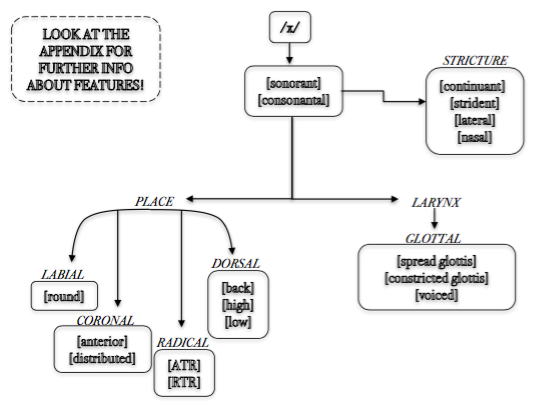
\includegraphics[scale=0.75]{features_tree}
\end{figure}

\ex. A {\bfseries natural class} is a grouping of sounds sharing one or more feature values. 
\begin{description}
\item {[}i, u]: [-consonantal, +sonorant, +high] 
\item {[}p, b, f, v, m]: [-consonantal, +round] 
\item {[}t, d, r, l, s, z, \textglotstop, \dh]: [+consonantal, -sonorant, +anterior] 
\end{description}
As we will see, identifying natural classes is important in phonology, since it leads to generalizing sound changes.

\subsection{Activity 1: Natural classes} 

{\itshape Each list below contains sounds all but one of which share some phonological property. Let?s find exactly one feature --- just one! --- that all the phones except one have and name the phone that is left out.}

\begin{enumerate}
\item {[i, e, u, k]}: /k/ is not a vowel (i.e., it is [+cons, -son])
\item {[t, d, g, b]}:
\item {[m, n, l, r]}:
\item {[\textipa{B}, ð, z, \textipa{G}]}:
\end{enumerate}

\subsection{Activity 2: British English vs American English}

{\itshape British and American speakers pronounce the following words in a slightly different way. Help me put the correct American pronunciation in the right-hand column of the table below.}

\begin{center}
\begin{tabular}{l c  | c | c}
	&	{\bfseries word}		&	{\bfseries British English}	&	{\bfseries American English} \\ \hline
a.	&	pure				&	[pju\textlengthmark\textschwa]	&						\\
b.	&	cute				&	[kju\textlengthmark t]			&						\\
c.	&	tune				&	[tju\textlengthmark n]			&						\\
d.	&	abuse			&	[\textschwa bju\textlengthmark s] &						\\
e.	&	dues				&	[dju\textlengthmark z]		&						\\
f.	&	argue			&	[\textscripta\textlengthmark gju\textlengthmark] &			\\
g.	&	muse			&	[mju\textlengthmark z]		&						\\
h.	&	new				&	[nju\textlengthmark]			&						\\
i.	&	lewd				&	[lju\textlengthmark d]			&						\\
j.	&	few				&	[fju\textlengthmark]			&						\\
k.	&	view				&	[vju\textlengthmark]			&						\\
l.	&	enthuse			&	[\textipa{InTju}\textlengthmark z] &						\\
m.	&	suit				&	[sju\textlengthmark t]			&						\\
n,	&	hue				&	[hju\textlengthmark]			&						\\
\end{tabular}
\end{center}	

{\itshape As you may yet have noticed, BE {\normalfont [ju]} is sometimes replaced by {\normalfont [u]} in AE --- but when? Let's list the context(s) in which this happens, and then try to group them in one natural class. \\

Your answer:}

\vspace{0.5cm}


\section{Abstractness level 2 -- fundamental notions}

\ex. A {\bfseries phone} is any speech sound.
\ex. A {\bfseries phoneme} is a phone used in a given language to form {\itshape minimally contrastive} words. Two sounds are two distinct phonemes when they occur in the same environment, hence their occurrence cannot be predicted any.
\a.[$\rightarrow$] Think of {\itshape diamonds}. When comparing the quality of two diamonds, they are typically compared with a black surface behind them. This is because the black surface provides a neutral background to highlight the contrast of the diamonds. In the same way, shared environments in words allow us to see more clearly that the two segments in question contrast with each other. Allophones are variants of the same phoneme.

\ex. The {\bfseries minimal pair test} is the only safe way to uncover the nature of sounds in a given language, since it helps us assess whether a pair of sounds are two different phonemes or allophones of the same phoneme in that language.

\begin{figure}[H]
\centering
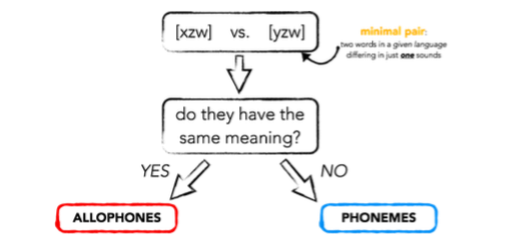
\includegraphics[scale=0.75]{minimal_pairs}
\end{figure}

\newpage

\subsection{Activity 3: Finding English phonemes}

{\itshape For each of the following pair of sounds, find out whether or not they are phonemes.}

\begin{center}
\begin{tabular}{c | c | c}
{\bfseries Pair} & {\bfseries Words} & Phonemes? (Y/N) \\ \hline
{[b] $\sim$ [p]}	&	buy $\sim$ pie	&			\\
{[f] $\sim$ [v]}	&				&			\\
{[e] $\sim$ [\textepsilon]}	&				&			\\
{[i] $\sim$ \textipa{I}]}		&				&			\\
{[p] $\sim$ [p\textsuperscript{h}]}	&				&			\\
\end{tabular}
\end{center}

\ex. Allophones may occur:
\a. in {\bfseries free distribution}, when they may appear in the same environment without a change in meaning and without being considered incorrect by speakers; or,
\b. in {\bfseries complementary (or contextual) distribution}, when they appear in two different phonological contexts; this means that their occurrence is \underline{predictable}.
	\a.[$\rightarrow$] Think of superheroes --- let's say my favorite, {\itshape Daredevil}. In reality, Daredevil and Matt Murdock are the same person. However, depending on the environment, you're going to see only one representation of Bruce Wayne --- you'll never see Daredevil and Matt Murdock hanging out in the same place at once.

\subsection{Activity 4: English aspirated stops}\label{aspirated_english}

{\itshape Analyze the English words in the table below: some stops show aspiration, some others do not. Can we identify the context in which each of them occurs? Complete the {\normalfont phonological rule} below.}

\begin{center}
\begin{tabular}{c | c || c | c}
{\bfseries Aspirated} 	& 	{\bfseries IPA} 	&	{\bfseries Unaspirated}	&	{\bfseries IPA} \\ \hline
pot 	&	[p\textsuperscript{h}\textscripta t]	&	spot					&	[sp\textscripta t] \\
top	&	[t\textsuperscript{h}\textscripta p]	&	stop					&	[st\textscripta p] \\ 
cot	&	[k\textsuperscript{h}\textscripta t]	&	Scot					&	[sk\textscripta t] \\
cat	&	[k\textsuperscript{h}\textipa{A}t]	&	guest				&	[g\textepsilon st] \\
tame 	&	[k\textsuperscript{h}e\textipa{I}m]		&	drain			&	[dre\textipa{I}n] \\
kite	&		[k\textsuperscript{h}e\textipa{I}t]		&	lucky			&	[l\textipa{2}ki] \\
\end{tabular}
\end{center}

\begin{figure}[H]
\centering
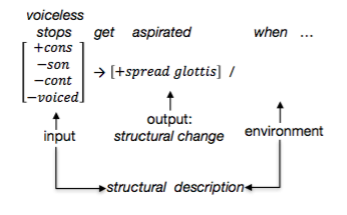
\includegraphics[scale=0.75]{phonorule}
\end{figure}

\subsection{Major phonological operations}

\ex. A sound may {\bfseries assimilate} to a neighboring sound with respect to some phonetic property (i.e., voicing, place of articulation and/or manner of articulation).

\subsubsection{Activity 5a: Assimilation (I)}

{\itshape In the following word chunks, consider the sound in bold. What sound do you actually produce?}

\begin{enumerate}
\begin{multicols}{3}
	\item I ca{\bfseries n} ask [...] 
	\item I ca{\bfseries n} bake [...] 
	\item I ca{\bfseries n} go [...]

\columnbreak

	\item ha{\bfseries t} trick [...]
	\item hi{\bfseries t} batsman [...] 
	\item nigh{\bfseries t} class [...]
	
\columnbreak

	\item ba{\bfseries d} dream [...] 
	\item hea{\bfseries d} band [...] 
	\item ba{\bfseries d} guy [...]
\end{multicols}
\end{enumerate}
	
\subsubsection{Activity 5b: Assimilation (II)}

{\itshape Consider the following forms of the English past tense. Do you always produce the same sound for the morpheme --{\normalfont ed}?}

\begin{center}
\begin{tabular}{ l l | l l }
abridged & [\textipa{@brI\textdyoghlig d}] & flagged & [fl\ae gd] \\
asked & [\ae skt] & claimed & [kle\textipa{I}md] \\
jumped & [\textdyoghlig\textipa{2}mpt] & typed & [ta\textipa{I}pt] \\
rubbed & [r\textipa{2}bd] & expressed & [\textepsilon kspr\textepsilon st] \\
\end{tabular}
\end{center}

\newpage

\ex. A sound may {\bfseries dissimilate} --- i.e. lose some phonetic property shared with an adjacent sound. For example, in the Latin adjectival suffix {\itshape -alis}, [l] dissimilates to [r] if another [l] is present nearby:

\vspace{-1em}

\begin{center}
\begin{tabular}{l l | l l}
nav-a{\bfseries l}is & `naval' & episcop-a{\bfseries l}is & `episcopal' \\
so{\bfseries l}-a{\bfseries r}is & `solar' & mi{\bfseries l}it-a{\bfseries r}is & `military' \\
{\bfseries l}upan-a{\bfseries r}is & `whorish' & ocu{\bfseries l}-a{\bfseries r}is & 'ocular' \\
\end{tabular}
\end{center}

\ex. A sound may be {\bfseries inserted} in a specific phonetic context. For example, consider the following words and expressions in Italian. 

\vspace{-1em}

\begin{center}
\begin{tabular}{l l | l l}
{[}princ{\itshape e}tonn{\itshape e}] & `Princeton' & {[}appl{\itshape e}] & `apple' \\
{[}njujork{\itshape e}] & `New York' & {[}in {\itshape i}spa\textltailn\textltailn a] & `in Spain' \\
\end{tabular}
\end{center}

\ex. A sound may be {\bfseries deleted} in a specific phonetic context. For example, in Italian [n] drops when followed by a consonantal cluster [sC]:

\vspace{-1em}

\begin{center}
\begin{tabular}{l c l l }
/i\underline{n}{\itshape st}allare/ & $\rightarrow$ & {[}i\underline{\hspace{0.1cm}}stallare] & `to install' \\
/i\underline{n}{\itshape st}ruttsjone/ & $\rightarrow$ & {[}i\underline{\hspace{0.1cm}}struttsjone] & `education' \\
/co\underline{n}{\itshape st}ruttsjone/ & $\rightarrow$ & {[}co\underline{\hspace{0.1cm}}struttsjone] & `construction' \\
\end{tabular}
\end{center}

\ex. Sounds may re-arrange in a specific context ({\bfseries metathesis}). For example, consider the following mispronunciations of English words.

\vspace{-1em}

\begin{center}
\begin{tabular}{l l | l l}
cavalry & [k\ae\textipa{lv@ri}] & foliage & [\textipa{fOIlI\textdyoghlig}] \\
comfortable & [\textipa{k2mft@rb@l}] & relevant & [\textipa{rEv@l@nt}] \\
asterisk & [\ae\textipa{st@rIks}] & prescription & [\textipa{p@rskrIpS@n}] \\
\end{tabular}
\end{center}

\ex. A segment may be produced more prominently in specific contexts ({\bfseries fortition}). Go back to the Activity in sec. \ref{aspirated_english} and review the data in the light of this new notion.

\ex. A segment may be produced less prominently in specific contexts ({\bfseries lenition}). The activity in sec \ref{flapping_english} below will be an example --- please hold on for the moment.

\subsection{Morphology 101}

\ex. A {\bfseries morpheme} is the smallest meaningful morphological unit of a given language.
\a. {\bfseries root}: the part of a word carrying the core meaning: e.g., \underline{table}-s; \underline{link}-ing 
\b. {\bfseries bound morphemes}: parts of a word that cannot occur alone, rather need to be attached to a root.
	\a. prefixes, occurring before a root: {\itshape im}-possible; {\itshape re}-iterate
	\b. infixes, occurring inside a root: wel-{\itshape diddly}-elcome (Ned Flanders)
	\c. suffixes, occurring after a root: talk-{\itshape ing}; driv-{\itshape er}

\ex. {\bfseries Allomorphs} are (contextual) variants of the same morpheme.

\subsubsection{Activity 6a: English plurals (I)}

{\itshape Look at the following list of English nouns; specifically, focus on the corresponding transcriptions of the plural forms. How many allomorphs conveying plurality can you identify? List them below, together with the context in which each of them occurs respectively.}

\begin{center}
\begin{tabular}{l | l || l | l}
{\bfseries singular} 	&	{\bfseries IPA}	&	{\bfseries plural}	&	{\bfseries IPA} \\ \hline
cat				&	[k\ae t]		&	cat-s				&	[k\ae ts]			\\
deed				&	[di\textlengthmark d]	&	deed-s		&	[di\textlengthmark dz] \\
tag				&	[t\ae g]			&	tag-s			&	[t\ae gz]			\\		
neck				&	[n\textepsilon k]		&	neck-s		&	[n\textepsilon ks]	\\
soap				&	[so\textipa{U}p]		&	soap-s		&	[so\textipa{U}ps]	\\	
pub				&	[p\textscripta b]		&	pub-s		&	[p\textscripta bz]	\\
wreath			&	[ri\textipa{T}]		&	wreath-s		&	[ri\textipa{T}s]		\\
ball				&	[b\textipa{O}l]		&	ball-s		&	[b\textipa{O}lz]		\\
computer			&	[k\textipa{2mpjiuR@r}]	& computer-s	&	[k\textipa{2mpjiuR@r}z] \\
boy				&	[b\textipa{OI}]		&	boy-s		&	[b\textipa{OI}z]		\\			
proof				&	[pruf]				&	proof-s		&	[prufs]			\\
clam				&	[kl\ae m]			&	clam-s		&	[kl\ae mz]			\\
can				&	[k\ae n]			&	can-s		&	[k\ae nz]			\\
myth				&	[\textipa{mIT}]		&	myth-s		&	[\textipa{mITs}]		\\
fly				&	[\textipa{flaI}]		&	fli-es			&	[\textipa{flaIz}]		\\
veto				&	[\textipa{viRoU}]	&	veto-es		&	[\textipa{viRoUz}	\\		
glass				&	[gl\ae s]			&	glass-es		&	[gl\ae s\textschwa z] \\
wish				&	[\textipa{wIS}]		& 	wish-es		&	[\textipa{wIS@z}]	\\
bus				&	[b\textscripta s]		&	bus-es		&	[b\textscripta s\textschwa z] \\
\end{tabular}
\end{center}

{\itshape Allomorphs for the English plural:} \\
\begin{enumerate}
	\item	
	\item
	\item
\end{enumerate}

\newpage

\section{Abstractness level 3: beyond the veil of Maya}

\ex. In phonology, the {\bfseries underlying representation} (UR) of a word or morpheme is the abstract form that a word or a morpheme is assumed to have before any (morpho-)phonological rules have applied to it. Accordingly, it is the form stored in the lexicon.

\ex. Conversely, the {\bfseries surface representation} (SR) is the phonetic realization of a given word or morpheme.
	\a.[$\rightarrow$] Hence: URs are made up of phonemes, SRs of (allo-)phones.

\ex. The {\bfseries derivation} is the road taken by an UR to come to surface; along this way, it may undergo some (morpho-)phonological change(s), governed by {\bfseries rules}. They usually need be applied in a specific {\itshape ordering} to get the desired surface form.
	\a.[$\rightarrow$] Let's think of Daredevil again. Matt (Murdock) would be the underlying representation, whereas Daredevil the surface representation after the `masking rule' applies.

\begin{figure}[H]
\centering
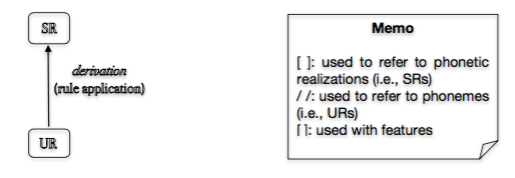
\includegraphics[scale=0.75]{phonoprocess}
\end{figure}

\begin{tcolorbox}

\begin{center}
{\bfseries {\itshape The long road beyond the veil of Maya} \\
how to identify what lies behind the surface}
\end{center}

\begin{enumerate}
	\item Identify the sound variation: what are the alternating phones?
	\item List the environment where each alternant occur:  what sounds surrounds them? Some formalisms:
		\begin{enumerate}
			\item word-initially: \#\_
			\item word-finally: \_\#
			\item between two vowels (any): V\_V
			\item between two consonants (any): C\_C \\ The space \_ is where the sound you are analyzing occurs.
		\end{enumerate}
\item Do (some of) the sounds occur in the same exact environment?
	\begin{enumerate}
		\item If so, and the two corresponding words have two different meanings, it means that the two sounds are in a {\itshape contrastive distribution}, i.e. they are phonemes;
		\item If so, and the two corresponding words have the same meaning, it means that the two sounds are allophones in {\itshape free variation};
		\item If not, the two sounds are {\itshape allophones distributing complementarily} depending on the phonological context. 
	\end{enumerate}
\item[] Now you have identified the kind of relationship between them, you can focus on the next step. In case of contrastive or free allophonic distribution, your job is done: there is no predictability power in such cases. In case of complementary distribution, you need to classify the environments in which each allophone occurs.
\item Once you have found the context in which each alternating sound occurs, you can work on stating the rule.
	\begin{enumerate}
		\item[$\rightarrow$] This is the {\bfseries trick}: in cases of complementary allophonic distributions, usually just one of the (two or more) alternants typically occurs in an environment that cannot be easily grouped in a {\itshape natural class} --- this hints that sound is likely to be the underlying representation!
	\end{enumerate}
\item Once you stated the rule, test your hypothesis by applying your rule(s) to the alleged UR. If you have detected more than one rule, you also want to check whether or not their application needs to be {\itshape ordered} in a specific way in order to get the desired surface representation.
\end{enumerate}

\end{tcolorbox}


\subsection{Activity 6b: English plurals (II)}

{\itshape Look again at data in table in Activity 4a above. Since plurality is just one piece of morphological information, in (morpho-)phonology we usually assume that it must be underlyingly present in just one form. Let's try to detect it, by using the box in the previous page.}

\begin{enumerate}
\item Alternating allomorphs: 
	\begin{enumerate}
		\item
		\item
		\item
	\end{enumerate}
\item Occurring environments:
	\begin{enumerate}
		\item 
		\item 
		\item 
	\end{enumerate}
\item What kind of alternation is that?
	\begin{enumerate}
		\item contrastive distribution
		\item free allophonic distribution
		\item complementary allophonic distribution
	\end{enumerate}
\item Phonological analysis:
	\begin{enumerate}
		\item By looking at the environment in which each allomorph occurs, which one do you is more likely to be the underlying form for the plural?
			
			\begin{figure}[H]
			\centering
			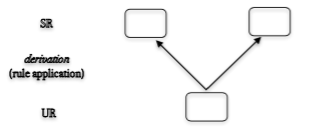
\includegraphics{plurals_ex}
			\end{figure}
\clearpage
		\item Finally, let's check rule ordering: does it matter? Complete the derivation in the table below. The goal is to apply all the rules we have just assumed in the same order for any word you possibly think of --- and still get the desired SR.
	\end{enumerate}
\end{enumerate}

\begin{center}
\begin{tabular}{r || c | c | c |}
{\itshape UR} 	& [k\ae t-\underline{\hspace{0.3cm}}] & [t\ae g-\underline{\hspace{0.3cm}}] & [\textipa{wiS}-\underline{\hspace{0.3cm}}] \\ \hline
			&							&							&								\\ \hline
			&							&							&								\\ \hline
{\itshape SR} 	& [k\ae t-s] & [t\ae gz] & [\textipa{wiS}\textschwa z] \\ \hline
\end{tabular}
\end{center}
	
\subsection{Activity 7: English flapping}\label{flapping_english}

{\itshape In table below alveolar stops {\normalfont /t, d/} become the alveolar flap {\normalfont [\textipa{R}]} in a specific context: what is that? State it below. }

\begin{center}
\begin{tabular}{c | c || c | c}
{\bfseries word}		& 	{\bfseries IPA}		& 	{\bfseries word}		& 	{\bfseries IPA} \\ \hline
ladder			&	[\textprimstress l\ae\textipa{R@}r]	&	latter				&	[\textprimstress l\ae\textipa{R@}r] \\	
soda				&	[\textprimstress s\textipa{oUR@}]	&	cider				&	[\textprimstress s\textipa{aIR@r}] \\
hitter				&	[\textipa{"hIR@r}]	&	etiquette			&	[\textipa{"ER@""kEt}] \\
stack				&	[\textprimstress st\ae k]			&	table				&	[\textprimstress t\textsuperscript{h}b\textschwa l]\\
\end{tabular}
\end{center}

\noindent {\itshape Now let's look at the additional data below. Do they contradict our first guess? If so, try to hone the rule you just stated. Hint: Look at the stress! Where does it fall?}

\begin{center}
\begin{tabular}{c | c || c | c}
{\bfseries word}		& 	{\bfseries IPA}		& 	{\bfseries word}		& 	{\bfseries IPA} \\ \hline
proton			&	[\textipa{proU''t\textsuperscript{h}\textscripta n}]	&	rattle			&	[\textprimstress r\ae\textipa{R@}l] \\	
rider			&	[\textprimstress \textipa{aIR@r}]	&	radar			&	[\textprimstress r\textipa{eId\textscripta r}] \\
retain				&	[\textipa{r@"\textsuperscript{h}eIn}]	&	material		&	[\textipa{m@t\textsuperscript{h}Irj@l}] \\
atom			&	[\textipa{"\ae R@m}]			&	atomic				&	[\ae\textprimstress t\textsuperscript{h}\textscripta \textipa{mIk}]\\
\end{tabular}
\end{center}

\noindent {\itshape Complete the following rule:}

\begin{center}
\phonc{\phonfeat{+cons \\
			 +anterior \\
			 -distributed}}{\phonfeat{+sonorant}}{\underline{\hspace{2cm}}}
\end{center}

\vspace{0.2cm}

\noindent {\itshape The data in the table above shows that in English alveolar flapping interacts with another phenomenon that we have just seen in one of the activities above: what is that? In which order do they have to apply? Remember that such order must be fixed, and account for all relevant data presented above. Complete the table below.}

\begin{center}
\begin{tabular}{r || c | c |}
{\itshape UR} 	& [\textipa{"\ae t@m}] & [\ae\textprimstress t\textsuperscript{h}\textscripta \textipa{mIk}] \\ \hline
			&							&							\\ \hline
			&							&							\\ \hline
{\itshape SR} 	& [\textipa{"\ae R@m}] & [\ae\textprimstress t\textsuperscript{h}\textscripta \textipa{mIk}] \\ \hline
\end{tabular}
\end{center}

\newpage

\subsection{Activity 8: Indonesian prefixes}

{\itshape Analyze the following Indonesian words into their constituent morphemes, and work out an underlying representation for each morpheme and each word.}

\begin{center}
\begin{tabular}{l | l | l | l}
	&	{\bfseries gloss}	&	{\bfseries simple form}	&	{\bfseries prefixed form} \\ \hline
a.	&	`throw'			&	lempar				&	l\textschwa lempar		\\
b.	&	`feel'				&	rasa					&	m\textschwa rasa		\\
c.	&	`represent'		&	wakil					&	m\textschwa wakili		\\
d.	&	`convince'			&	yakin					&	m\textschwa yakin		\\
e.	&	`cook'			&	masak				&	m\textschwa masak		\\
f.	&	`marry'			&	nikah				&	m\textschwa nikah		\\
g.	&	`chat'			&	\ng aco				&	m\textschwa\ng aco		\\
h.	&	`sing'			&	\textltailn a\textltailn i		&	m\textschwa\textltailn a \textltailn i \\	
i.	&	`count'			&	hitu\ng				&	m\textschwa\ng hitu\ng		\\
j.	&	`draw'			&	gambar				&	m\textschwa\ng gambar		\\
k.	&	`send'			&	kirim					&	m\textschwa\ng irim			\\
l.	&	`hear'			&	d\textschwa\ng ar		&	m\textschwa nd\textschwa\ng ar \\
m.	&	`write'			&	tulis					&	m\textschwa ntulis	\\
n.	&	`help'			&	bantu				&	m\textschwa mbantu		\\
o.	&	`hit'				&	pukul				&	m\textschwa mpukul		\\
p.	&	`sew'				&	\textyogh ahit			&	m\textschwa\textltailn\textyogh ahit \\
q.	&	`note down'		&	\textteshlig atat			&	m\textschwa\textltailn\textteshlig atat	\\
r.	&	`take'			&	ambil				&	m\textschwa\ng ambil	\\
s.	&	`fill up'			&	isi					&	m\textschwa\ng isi	\\
t.	&	`invite'			&	unda\ng				&	m\textschwa\ng unda\ng	\\
\end{tabular}
\end{center}

\begin{enumerate}
{\itshape
	\item What is the underlying form of the prefix? Why?
	
	\vspace{1cm}
	
	\item List the underlying representations of any other alternating morphemes (hint: look at changes in the roots!).
	
	\vspace{1cm}
	
	\item Let's try to list all the rules we need to assume, given the corpus above; do they need to be ordered somehow? Complete the derivations in the table below.
}
\end{enumerate}

\begin{center}
\begin{tabular}{r || c | c | c | c |}
{\itshape UR} 	& [\underline{\hspace{0.5cm}}-ambil] & [\underline{\hspace{0.5cm}}-bantu] & [\underline{\hspace{0.5cm}}-lempar] & [\underline{\hspace{0.5cm}}-tulis] \\ \hline
			&							&							&							    &							\\ \hline		
			&							&							&							    &							\\ \hline 	
			&							&							&							    &						\\ \hline
{\itshape SR} 	& [m\textschwa\ng ambil] & [m\textschwa mbantu] & [m\textschwa lempar] & [m\textschwa n-tulis] \\ \hline
\end{tabular}
\end{center}

\section{Recap}

\ex. {\itshape Phonology} studies the linguistic sounds a given language makes use of, to make up words. Phonology also looks at sound changes occurring in specific phonological and morphological contexts.

\ex. To explain such changes, phonologists use {\itshape features}, i.e. specific articulatory configurations; they are usually assumed to have binary values: [+] indicates the presence of a specific articulatory movement, [-] indicates its absence. Changes are explained as phenomena occurring exclusively in sounds that can be grouped together as sharing at least one feature value ({\itshape natural classes}).

\ex. {\itshape Minimal pair testing} is the only way to figure out whether two phones are used {\itshape contrastively} in a given language. Only if a minimally different pair of words conveys two different meanings, the two different sounds are to be considered as phonemes in that language; otherwise, one is an allophone of the other.

\ex. Phonological operations include: {\itshape assimilation, dissimilation, insertion, deletion, metathesis, fortition, lenition}.

\ex. Occurrence of phonological operations implies the presence of an abstract level of representation of sounds ({\itshape underlying representation}), which may undergo specific (morpho-)phonological operations leading to a phonetic representation ({\itshape surface representation}). {\itshape Ordering of rules} is sometimes crucial, in order for the underlying representation to surface as expected.

\newpage

\thispagestyle{empty}

\appendix

\section{Little Handbook of phonological features}

\begin{tcolorbox}
\small
\begin{center} --- {\scshape Root Tier} --- \end{center}
\vspace{-2em}
\begin{description}
	\item[{[consonantal]}] constriction in the vocal tract. [+consonantal] are obstruents, nasals, liquids, and trills; vowels are [-consonantal].
	\item[{[}sonorant{]}] type of oral constriction that can occur in the vocal tract. [+son] designates the vowels and sonorant consonants (namely glides, liquids, and nasals), which are produced so that the air pressure in the vocal tract is the same as the external air pressure; [-son] alternatively describes obstruents, characterized by an imbalance of air pressure in the vocal tract.
\end{description}
\vspace{-2em}

\begin{center} --- {\scshape Stricture Tier} --- \end{center}
\vspace{-2em}
\begin{description}
	\item[{[continuant]}] passage  of  air  through  the  vocal  tract.  [+cont]  are  mainly  fricative  sounds;   stops  are typically [-cont].
	\item[{[strident]}] a type of friction that is noisier than usual. This is caused by high energy white noise.
	\item[{[lateral]}]	the shape and positioning of the tongue with respect to the oral tract. In [+lat]  sounds the constriction occurs in the central area of the vocal trace, but the sides of the tongues are lowered so that air can pass through.
	\item[{[nasal]}]	the position (lowered/raised) of the velum. [+nasal] sounds are produced with a lowering of the soft palate, so that air can flow through the nasal cavity; in [-nas] sounds the velum is raised.
\end{description}
\vspace{-2em}

\begin{center} --- {\scshape Laryngeal Tier} --- \end{center}
\vspace{-2em}
\begin{description}
	\item[{[spread gl.]}] openness of the glottis. [+spr gl] sonorant sounds are  characterized by a breathy voice, non-sonorant [+spr gl] sounds are aspirated.
	\item[{[constricted gl.]}] degree of closure of the glottis. [+constr gl] sonorant sounds are characterized by a creaky voice, non-sonorant [+constr gl] sounds are glottalized.
	\item[{[voice]}] vibration of the vocal folds: voiced/unvoiced segments.
\end{description}
\vspace{-2em}

\begin{center} --- {\scshape Place Tier} --- \end{center}
\vspace{-2em}
\begin{description}
	\item[{[round]}]	[+round] sounds are produced with lip rounding, in [-round] sounds there is no such constriction.
	\item[{[anterior]}] anterior segments are articulated with the tip or blade of the tongue at or in front of the alveolar ridge.
	\item[{[distributed]}] for [+dist] segments the restriction is extended to an extended area on the median longitudinal axis of the vocal tract.
	\item[{[high]}] [+high] segments raise the tongue body close to the palate, [-high] segments do not.
	\item[{[low]}] [+low] segments bunch the tongue body to a position low in the mouth.
	\item[{[back]}] [+back] segments are produced with the tongue body bunched and retracted slightly to the back of the mouth; [-back] segments are bunched and extended slightly forward.
	\item[{[ATR]}] advanced position of the root of the tongue. For anatomical reasons, [+ATR] sounds usually are [+high] too.
	\item[{[RTR]}] retracted position of  the  root  of  the  tongue  towards  pharynx;  uvular   and  pharyngeal sounds are [+RTR].
\end{description}

\end{tcolorbox}

\section{Chart of phonological features}

\thispagestyle{empty}

\begin{figure}[H]
\centering
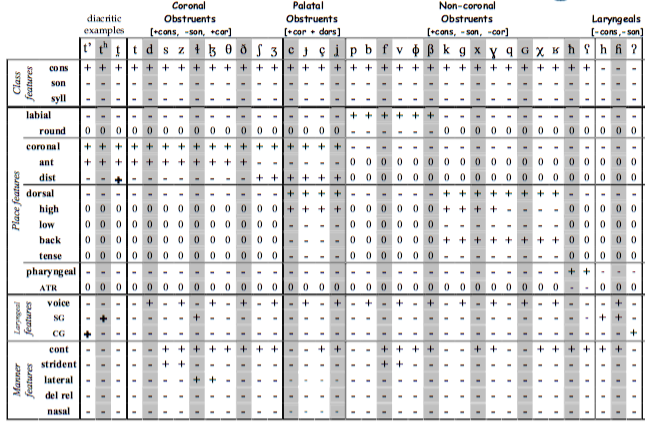
\includegraphics[scale=0.75]{chart_features_1}
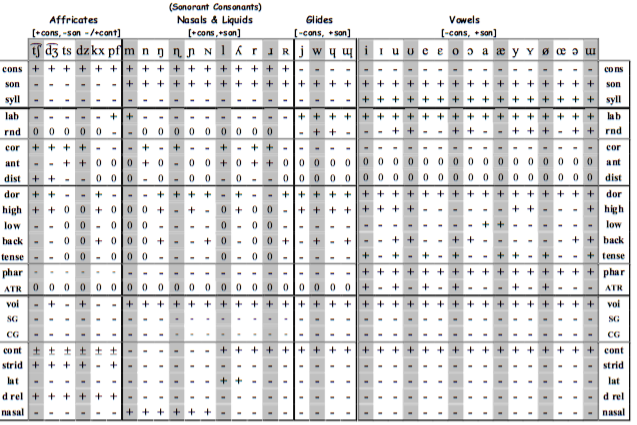
\includegraphics[scale=0.75]{chart_features_2}
\end{figure}

\end{document}